\documentclass[dvipsnames,a4paper,11pt]{article}

\usepackage[utf8]{inputenc}
\usepackage[T1]{fontenc}
\usepackage{a4wide}
\usepackage{amsmath}
\usepackage{todonotes}
\usepackage{xcolor}
\usepackage{amsthm}
\usepackage{amssymb}
\usepackage{accents}


\newtheorem{thm}{Theorem}
\newtheorem{prop}{Propery}

\theoremstyle{definition}
\newtheorem{defn}{Definition}

\theoremstyle{remark}
\newtheorem{rmq}{Remark}

\theoremstyle{remark}
\newtheorem{ex}{Example}

\newcommand{\tiph}[1]{\todo[inline,color=Orchid]{#1}}
\newcommand{\pimprenelle}[1]{\todo[inline, color=ForestGreen]{#1}}
\newcommand{\jeffin}[1]{\todo[inline, color=BrickRed]{#1}}
\newcommand{\jeff}[1]{\todo[color=BrickRed]{#1}}


\title{Multiplex stream graphs}
\author{Pimprenelle Parmentier, Tiphaine Viard, \ldots}

\begin{document}
    \maketitle

    \section{Multilayer stream graphs}

	\subsection{Definition}
    We define a multiplex stream graph as a tuple $M = (T,T_M,V,W_M,E_M,{\cal L})$, such that $T$ and $V$ are, respectively, a time interval and a set of nodes, just like for stream graphs \cite{stream}.
    As for multilayer graphs \cite{mlkiv}, ${\cal L}$ is a set of $d$ {\em aspects}; ${\cal L} = \{L_i\}_{i=1}^d$, and an element $\alpha_i$ of $L_i$ is named {\em elementary layer}. An element of $L=L_1\times \dots \times L_d$ is named {\em layer}.

	$T_M$ is a set of intervals of $T$ so for that each layer $\alpha$, $T_{\alpha}$ is the interval at which the layer exists. For each $t$ in $T$, $\exists \alpha \in L | t \in T_{\alpha}$ (at any time, all the aspects are non-empty).

	$W_M \subseteq T\times V \times (L_1 \times \dots \times L_d)$ represents the existing points on layers with respect to time.

   $E_M \subseteq T\times V_M \otimes V_M$ are the links appearing with respect to time,  $V_M = \{ (u,\alpha), u\in V, \alpha \in L\}$. The elements of $V_M$ are named {\em node-layer}.

    Notice that just like in multiplex networks, nodes in time ({\em i.e.}, elements of $W_M$) can be present in an arbitrary number of layers.

   	\pimprenelle{La représentation de la présence ou non des couches en fonction du temps par $T_M$ est un choix, que nous préférons pour le moment à celle $M_M$ des couples $(t,\alpha)$}

	\subsection{2 examples}
	\begin{ex}[Research world]\label{exresearch}
	We consider a set of people working in research.
	
	These people can work in one or more universities and/or companies, in one or more departments. They can work together on different ways : they can collaborate on a paper, supervise or being supervised. And their work on different subjects, linked together thanks to keywords.


	The multilayer stream graph is the following :
	\begin{itemize}
		\item the {\bf nodes V} are the researchers
		\item the {\bf aspects L} are : the university/companies , the departments, the subjects, the type of status of interaction (supervisor/ supervised / collaborator) 
		\item {\bf links} appear during an interaction between two researchers.
		\item all these parameters vary with time, the set $T$ is chosen arbitrarily
	\end{itemize}
	
	Question : which aspect is the more important in the spreading and creation of knowledge ?
	
	\end{ex}
	
	\begin{figure}
    	\centering
    	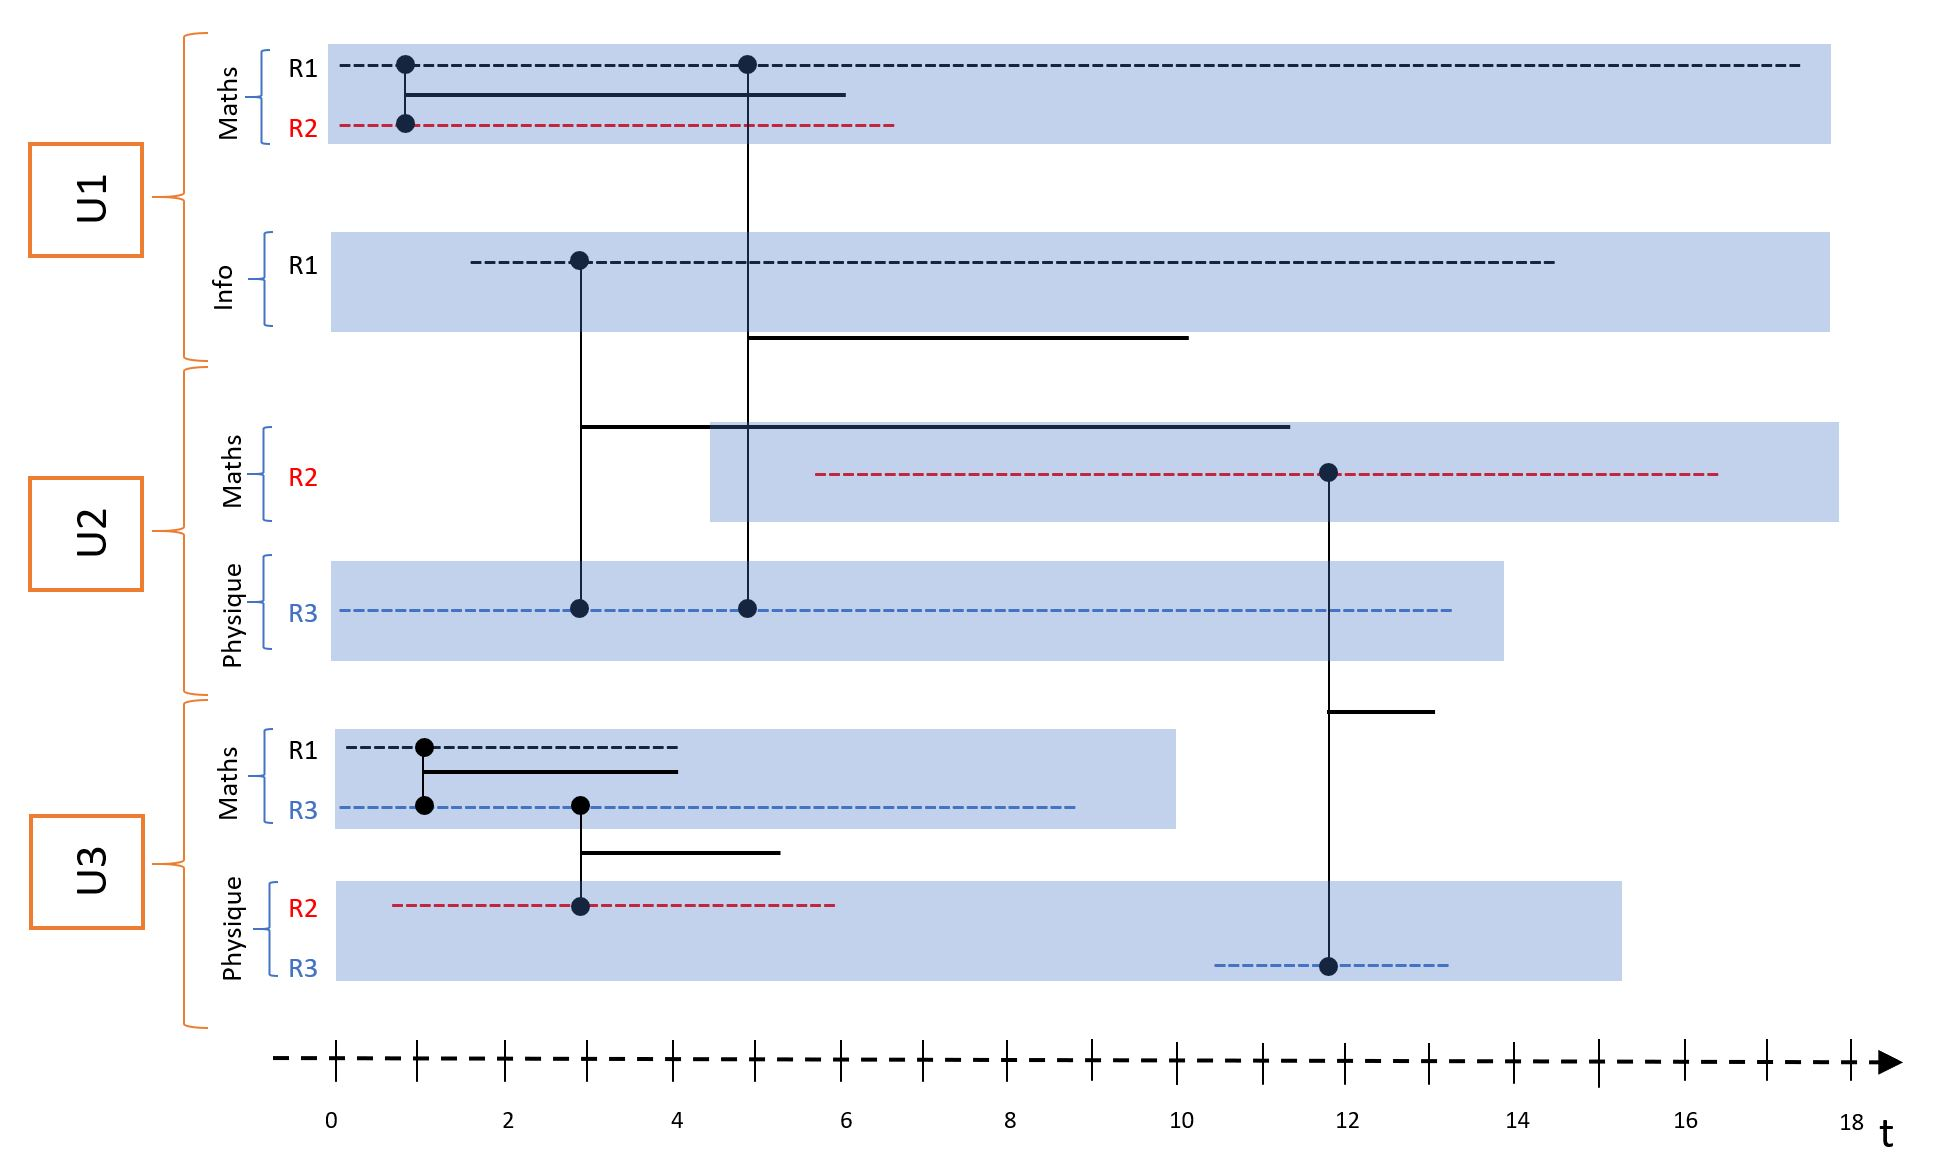
\includegraphics[width=15cm]{schemas/chercheurs.jpg}
    	\caption{An simplified scheme of a multiplex stream graph for example \ref{exresearch}. The nodes are the researchers R1,R2,R3, and the aspects are the Universities (U1,U2,U3), and the department (Maths, Computer sciences, Physics)}
    	\label{fig:chercheurs}
	\end{figure}
	

	\begin{ex}[Epidemics between species]
		We consider an set of individuals from different species, and a disease. This disease could be transmitted through different types of interaction : by blood, by  by respiratory tracts, digestive tracks, etc.
		
		The stream-multilayer graph is the following : 
		\begin{itemize}
			\item the {\bf nodes V} are the individuals
			\item the {\bf aspects L} are : the species, the type of possible interaction, the state of the individual (sane, infected, contagious, dead, recoved ... ) 
			\item {\bf links} appear when there is an interaction between two individuals.
			\item all these parameters vary with time, the set $T$ is chosen arbitrarily (from example from the start of the infection)
		\end{itemize}
	
		The question here could be : when and where do we have to act (cut some connection / remove some node-layer) to stop the spreading of the disease as soon as possible ?
	\end{ex}

	
	\begin{rmq}
		We notice that it is easy to make the multilayer as complex as we want. Three rules seem to be important to have a pertinent use of multiplex-stream graph :
		\begin{itemize}
			\item a set of nodes which could have various properties which can be "melted"
			\item different ways to interact between the nodes in function of their properties
			\item a time-dependency
		\end{itemize}
	\end{rmq}
	
	
   	\subsection{Substreams and operations over substreams}

    From this definition, let us define common streams of interest.

	For any layer $\alpha \in L_1 \times \dots \times L_d$, the {\em intra-layer} stream graph $S^{\alpha}$ is the stream $S^{\alpha}=(T^{\alpha},V^{\alpha},W^{\alpha},E^{\alpha})$ such that for all $t$ in T :
	\begin{itemize}
		\item $T^{\alpha} = T_{\alpha} \in T_M$
		\item $V^{\alpha} =\{(u,\alpha),u\in V\} \cap V_M$
		\item $W^{\alpha} =\{(t,u,\alpha),|u\in V, t \in T \} \cap W_M$
		\item $E^{\alpha} = \{(t,(u,\alpha),(v,\alpha))| t \in T,(u,v)\in V^2 \} \cap E_M$.
	\end{itemize}


	For any two layers $\alpha, \beta \in L_1\times \dots\times L_d$, the {\em inter-layer} stream graph is the stream $S^{(\alpha,\beta)} = (T, V^{\alpha,\beta},W^{\alpha,\beta},E^{\alpha,\beta})$ such that :
	\begin{itemize}
		\item $T^{\alpha,\beta}=T^{\alpha}\cap T^{\beta}$
		\item $V^{\alpha,\beta} = \{u,\gamma | u \in V, \gamma \in \{\alpha,\beta\} \} \cap V_M$
		\item $W^{\alpha,\beta}= \{(t,u,\gamma) | u \in V, \gamma \in \{\alpha,\beta\} \} \cap W_M$
	    \item $E^{\alpha,\beta} = \{(t,(u,\alpha),(v,\beta) | u,v \in V\} \cap E_M $
	\end{itemize}

	    Notice that for any layer $\alpha$, $S^{(\alpha)}$ is equivalent to $S^{(\alpha,\alpha)}$.



	The {\em intersection} of two substreams $S_1$ and $S_2$ is defined as follows :
	\[
		S' = S_1 \cap S_2 = (T_1\cap T_2, V_1 \cap V_2, W_1 \cap W_2, E_1\cap E_2)
	\]

	Notice that this intersection is a stream graph too.

	The {\em union} of two substreams $S_1$ and $S_2$ is defined as follows :
	\begin{align*}
		S' = S_1 \cup S_2 = (T', V_1 \cup V_2, W_1 \cup W_2, E' \})\\
		T' = [\min(T_1,T_2),\max(T_1,T_2)]\\
		E' = E_1 \cup E_2 
	\end{align*}

	Notice that the union of two sub stream graphs gives a stream graph.

		\begin{prop}
		\[
			\bigcup_{(\alpha,\beta) \in L^2} S^{(\alpha,\beta)} = S_U(M)
		\]
	\end{prop}
	\begin{proof}
		\begin{align*}
			S=\bigcup_{(\alpha,\beta) \in L^2} S^{(\alpha,\beta)}\\
			S=(T^{*},V^{*},W^{*},E^{*})\\
			S_U(M) = (T_U,V_U,W_U,E_U)			
		\end{align*}		 
	
	
	\begin{itemize}
		\item $T=T_U$ by definition of $S_U$. Let's take $t\in T$. By definition of multilayer stream graphs, $\exists \alpha \in L | t\in T_{\alpha}=T^{\alpha,\alpha}$. So $t \in [\underset{(\alpha,\beta) \in L^2}{\min}(T^{\alpha,\beta}),\underset{(\alpha,\beta) \in L^2}{\max}(T^{\alpha,\beta})]=T^{*}$. $T_U \subseteq T^{*}$. 
	Moreover, $\underset{(\alpha,\beta) \in L^2}{\min}(T^{\alpha,\beta}) \geq \min(T)$ 
	and $\underset{(\alpha,\beta) \in L^2}{\max}(T^{\alpha,\beta}) \leq \max(T)$. 
	So $\mathbf{T^{*} = T}$.
		\item  $V_M = V_U$ by definition of $V_U$.$V^{*}=\bigcup_{(\alpha,\beta) \in L^2} V^{\alpha,\beta} \subseteq V_M$.
	Let $(v,\alpha) \in V_U$. $(v,\alpha) \in V^{\alpha,\alpha} \in V^{*}$.$V^{*}=V_U$.$\mathbf{V^{*}=V_U}$.
		\item $W_U=W_M$ and $W^{*}=\bigcup_{\alpha,\beta \in L^2} W^{\alpha,\beta} \subset W_M$. So as for all $ (t,u,\alpha)$ in $W_M$, $(t,u,\alpha)$ belongs to $W^{\alpha,\alpha}$, $W_M$ is a subset of $W^{*}$. So $\mathbf{W^{*}=W_M}$.
		\item $E_U=E_M$ and $E^{*}=\bigcup_{\alpha,\beta \in L^2}(E^{\alpha,\beta})$ by definition. So as $E^{\alpha,\beta}$ is a subset of $E_M$ for every couple of layers $\alpha,\beta$, $E^{*} \subset E_M$. 
		$\forall e =(t,u,\alpha,v,\beta) \in E_M$, $e \in E^{\alpha,\beta}$. So $\mathbf{E_M=E^{*}}$.
	\end{itemize}		
	\end{proof}


	\subsection{Projections }

    The {\em coupling edges} are $E_C=\{(t,u,\alpha,v,\beta)\in E_M | u=v\}$.

    The {\em intra-layer edges} are $E_I = \{(t,u,\alpha,v,\beta) \in E_M | \alpha = \beta \}$

    The {\em inter-layer edges} are $\bar{E_I} = E_M\backslash E_I$.
    
	(See fig.\ref{exIntraInter} for a visual representation.)
	
	\begin{figure}[h]
		\centering
		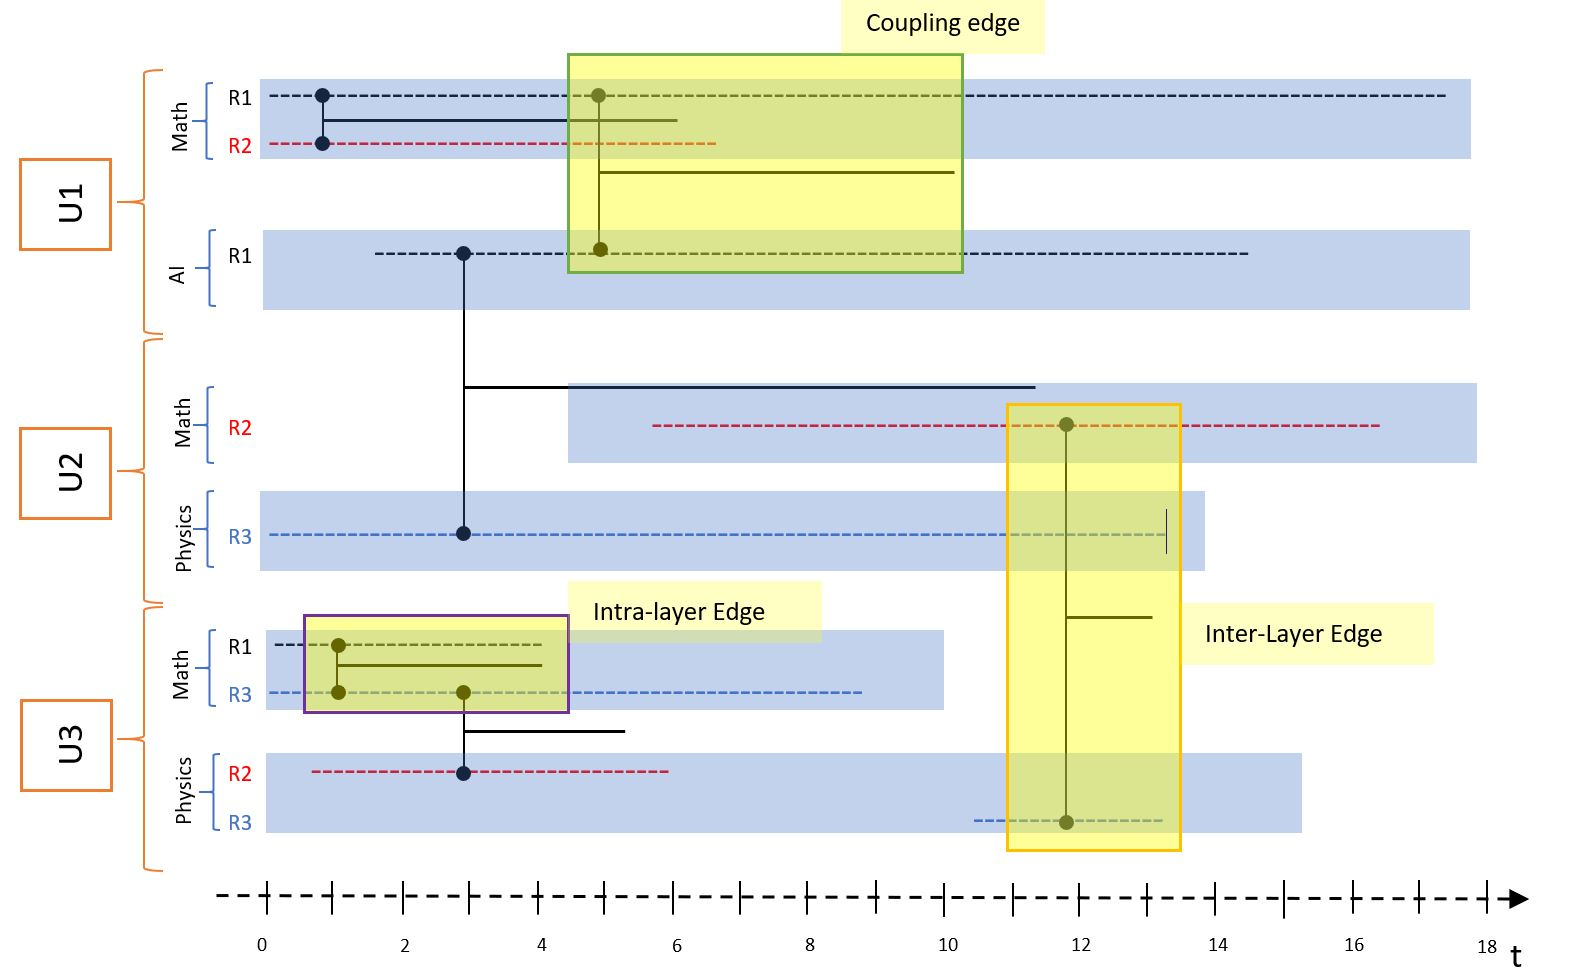
\includegraphics[width=\textwidth]{schemas/edgesCat.jpg}
		\caption{Illustration with our example of coupling edges, intra-layer edges and inter-layer edges}
		\label{exIntraInter}
	\end{figure}
   	The {\em multilayer graph at time t} $M_t$ is $M_t = (V_{M,t}, E_{M,t},V_t,{\cal L}_t)$ with :
    \begin{itemize}
		\item $V_{M,t} = \{(u,\alpha)| (t,u,\alpha)\in W_M\}$
		\item $E_{M,t} = \{(u,\alpha,v,\beta) | (t,u,\alpha,v,\beta) \in E_M\}$
		\item $V_t = {u | (t,u) \in V}$
		\item ${\cal L}_t = {L_i,t}_{i=1}^d, L_{i,t}=(\alpha)_i, t\in T_\alpha$
    \end{itemize}

	\begin{figure}[h]
		\begin{minipage}{0.49\linewidth}
			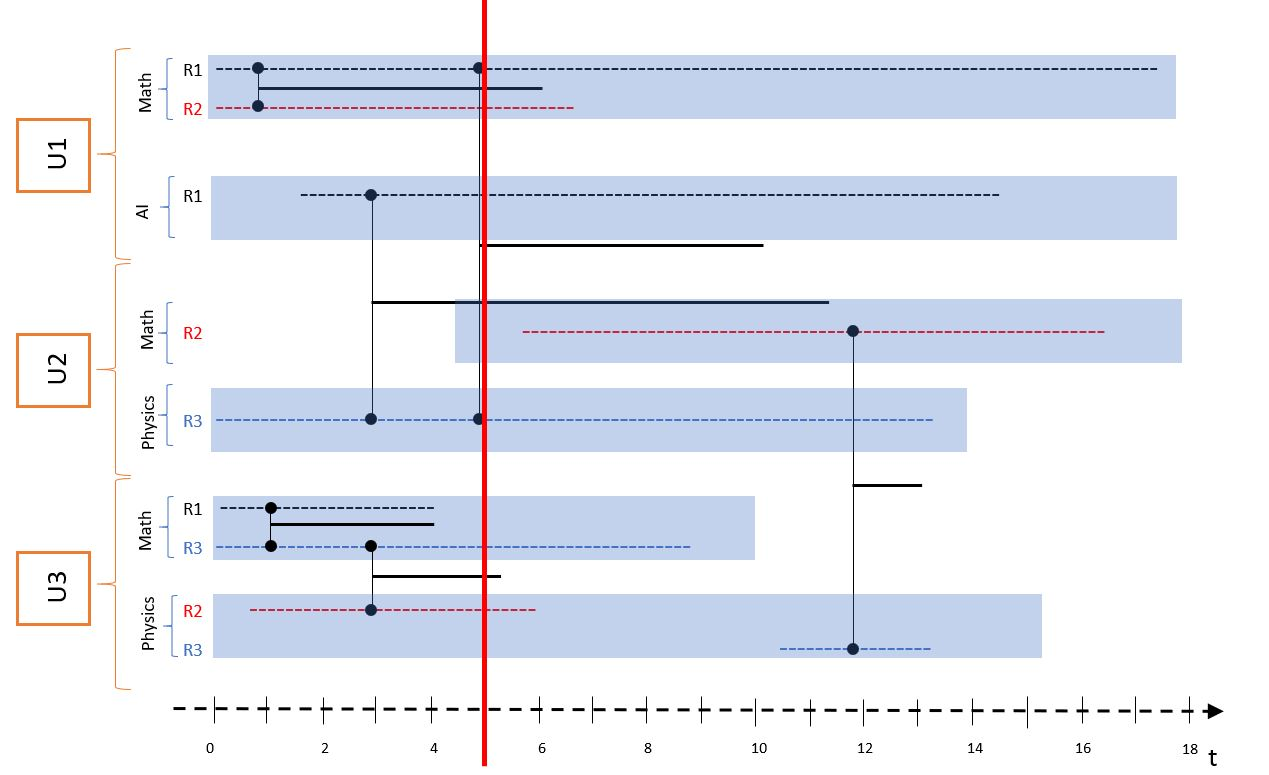
\includegraphics[width=\textwidth]{schemas/pauset.jpg}
		\end{minipage}
		\begin{minipage}{0.49\linewidth}
			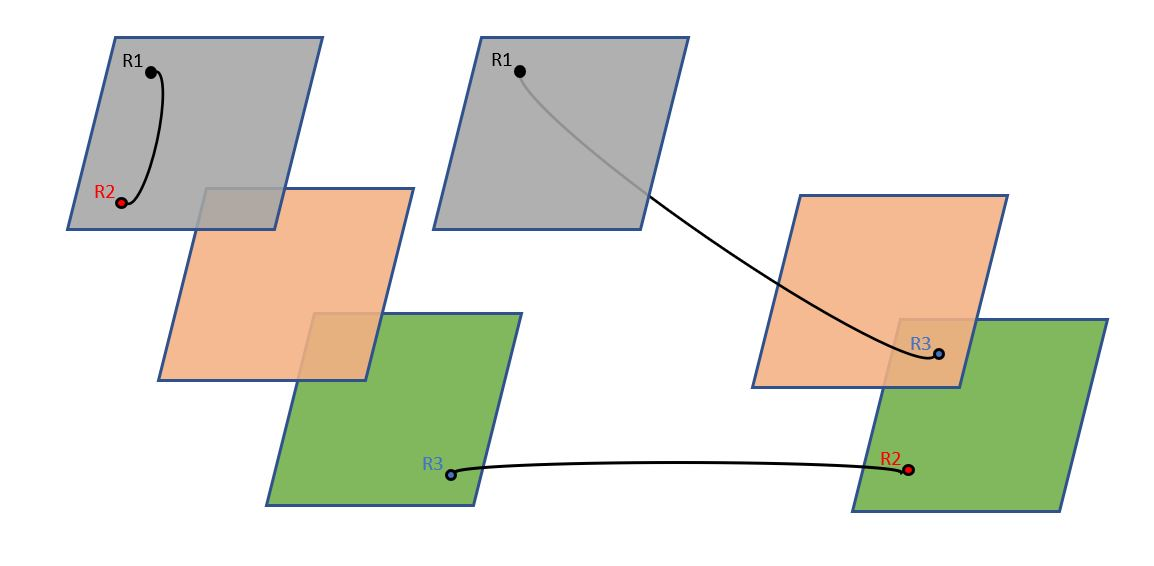
\includegraphics[width=\textwidth]{schemas/pausetproj.jpg}
		\end{minipage}
		\caption{Our multilayer example at time $t=5$}
	\end{figure}
	
    \begin{rmq}
    	We assume that $\forall (i,t), \; L_{(i,t)} \neq \emptyset$.
    \end{rmq}

    A {\em multiplex stream graph (MpSG)} is a graph in which the only inter-layer connections allowed are connections between the same point : $E_M = E_I \cup E_C$.

    The {\em multilayer graph induced} $M_I(M)$ of $M$ is the multilayer graph which gather all the points on all the layer who appear during $T$ and all the links in $E$.
    \begin{align*}
    	M_I(M) = (V_{M,I}, E_{M,I}, V_I,L_I)\\
    	V_{M,I} = \bigcup_{t\in T} V_{M,t}\\
    	E_{M,I} = \bigcup_{t\in T} E_{M,t}\\
    	V_I = \bigcup_{t\in T} V_t \\
    	L_I = \bigcup_{t\in T} L_t\\
    \end{align*}

    The {\em underlying stream } $S_U(M)$ of $M$ is $(T,V_M,W_M,E_M)$, and could be share into clusters corresponding to the different layers. This definition is a generalisation to the one used for simple multilayer graphs.




   

	


	\section{Number of nodes, number of layers}
	
	
	 The {\em contribution} of one node-layer in the MPG is $n_{v,\alpha} = \frac{|T_{v,\alpha}|}{|T|}$. The {\em number of node-layers} is the sum of the contributions $N(M) = \underset{(u,\alpha)\in V_M}{\sum} n_{(u,\alpha)} = \frac{|W_M|}{|T|}$.
    
**************NEW*******************    
    
    We define too the {\em contribution} of one layer as follows : $n_\alpha = \frac{|T_{\alpha}|}{|T|}$. The {\em number of layers is then the sum of the contributions}.
    
	In multilayer graphs, the number of nodes hasn't been fully defined as far as we know.
	Rather than just counting the nodes or the node layers, we define the {\em number of nodes in a multilayer} as :
	\begin{align*}
		N_{nodes in multilayers}(M_l) = \frac{\text{number of node-layers}}{\text{number of layers}}
	\end{align*}	    
	Notice that if there is only one layer, we find the classical number of nodes. A node appearing in half of the layers doesn't bring the same contribution than a node appearing in all the layers.  
    
    We decide then to define the \textbf{number of nodes} as follows : 
    
    The {\em the contribution} of a node describes the rate of appearance of the node on the different layers : $n_v = \frac{\sum_{\alpha \in L}|T_{v,\alpha}|}{\sum_{\alpha \in L} |T_{\alpha}|}$.
    The {\em number of nodes} is then the sum of the contribution of the nodes : 
    \begin{align}
    N_n(M) = \sum_{v\in V} n_v= \sum_{v\in V} \frac{\sum_{\alpha \in L}|T_{v,\alpha}|}{\sum_{\alpha \in L} |T_{\alpha}|} 
    \label{numberNodes}
	\end{align}     
**********END nEW*******************

	The {\em overlap presence } of two nodes-layers $(u,\alpha)$ and $(v,\beta)$ measures the rate of simultaneous presence of two node-layers :
	\begin{align*}
		\mathbb{U}((u,\alpha),(v,\beta))=\mathbb{P}( t \in T_{u,\alpha} \cap T_{v,\beta} | t \in T_{u,\alpha} \cup T_{u,\beta}) \\
		= \frac{|T_{u,\alpha}\cap T_{u,\beta}|}{|T_{u,\alpha}\cup T_{u,\beta}|}
	\end{align*}

	The {\em overlap presence} of two layers $\alpha$ and $\beta$ is defined on the same pattern :
	\begin{align*}
		\mathbb{U}(\alpha,\beta) = \frac{|T_{\alpha}\cap T_{\beta}|}{|T_{\alpha}\cup T_{\beta}|}
	\end{align*}

    The {\em node-layer uniformity} measures the rate of simultaneous presences of node-layers in the multilayer-stream graph :
    \[
    	\mathbb{U}(M) = \frac{\sum_{(u,\alpha),(v,\beta) \ V_M \otimes V_M}{|T_{(u,\alpha)} \cap T_{(v,\beta)}|}}{\sum_{(u,\alpha),(v,\beta) \ V_M \otimes V_M}{|T_{(u,\alpha)}\cup T_{(v,\beta)}|}}
    \]



	\begin{rmq}
		Note that this concept can be used for sub-stream graphs of any type.
	\end{rmq}

	When $\mathbb{U}=1$, we say that the multilayer stream graph is uniform.



    \section{Density}
	In classical graphs (unweighed and non directional), the density $d(G)$ measures how much the vertexes are connected.
		\[
			d(G) = \frac{|E|}{|V\otimes V|} = \frac{2\times |E|}{|V|(|V|-1)}
		\]
	In stream graphs, the density measures too the "rate of connectivity", or the probability that, at a randow time when two point exist, they are connected.

		\begin{align*}
			\delta_s(G) = & \mathbb{P}((t,u,v)\in E| (t,u),(t,v) \in W) \\
			 =  & \frac{\sum_{uv \in V \otimes V}{|T_{uv}|}}{\sum_{uv \in V\otimes V}{|T_u\cap T_v|}}= \frac{\int_{t\in T}{|E_t|dt}}{\int_{t\in T}{|V_t\otimes V_t|dt}}
		\end{align*}

	We can then define the density of the multilayer graph. Notice first that the density measures the rate of connectivity, and so depending to the type of system we study, the definition can change. If some connections are forbidden, we will ignore them in the density. We name $C \in V_M\times V_M$ the set of possible connections in the mutlilayer. If some connections are automatics (like the ones between the same node in different layers), we don't take it into account too.
	\[
		\delta_M (M) = \frac{|E_M|}{|\{\text{"possible connections"}\}|}
	\]

	The generalisation to multilayer stream graphs is then natural.
	\[
		\delta_M (M) = \frac{\int_{t\in T}|E_M,t|}{\int_{t\in T}|C|} = \frac{\sum_{(u,\alpha)(v,\beta) \in V_M \otimes V_M}|T_{(u,\alpha)(v,\beta)}|}{\sum_{(u,\alpha)(v,\beta) \in C}|T_{(u,\alpha)}\cap T_{(v,\beta)}|}
	\]

	For example, in a multiplex stream graph, $C=\{(t,u,\alpha),(t,v,\beta))| t\in T_{u,\alpha} \cap T_{u,\beta}, u=v \text{or} \alpha = \beta)\}$ :

	\[
		\delta_M (M) = 
		\frac{|E_M|}{|C|}= 
		\frac{\sum_{(u,\alpha)(v,\beta) \in (V_M \otimes V_M)} |T_{(u,\alpha)(v,\beta)}|}
		{(\sum_{\alpha \in L}\sum_{(u,v) \in V\otimes V}|T_{u,\alpha} \cap T_{v,\alpha}|)+( \sum_{u \in V } \sum_{(\alpha,\beta) \in L \otimes L}|T_{u,\alpha}\cap T_{u,\beta}|)}
	\]

		\section{Neighbours and degrees}
	
		In classic graphs, the degree of a node is the number of its neighbours. The neighbours are the nodes for which a link between the first node and the neighbour.
		
		\subsection{Nieghbours and degree in multilayer graphs}
		
		In the multilayer graphs, it is a more tricky question to know who are the neighbours of a node. In many multiplexes, the nodes-layers corresponding to the same node are linked together with an "invisible" connection. The main question should be of course : "what do we want to measure ?" We will give a few examples of different situation and the definition of the degree associated.
		
		I the case of a transportation multiplex, our nodes are some cities, the layers are different types of means of transportation. If we want to know how many cities you can reach from Tokyo without correspondence, we will calculate the degree of Tokyo in the aggregated graph.
		
		But we might want to highlight the fact that it is not equivalent to have one or many different links in different layers between two nodes. For example, two city will be better connected if we can take the train of the plane to travel between them.  We then can take the sub-multilayer graph of the neighbours of all the node-layers labelled Paris, and compute the number of nodes as defined in \ref{numberNodes}. 
		
		\begin{align}
			d_2(v)= \frac{|\{((u,\alpha,v,\beta) \in E\}|}{|L|} = \frac{\text{Number of node-layers neighbours of u}}{\text{number of layers}}
		\end{align}
		
		But this time, we lose the information of how many cities we can reach. A city connected to two other cities by the train will have the same score than a city connected to only one city by train and plane. The good point is just that if we have just one layer, we find again the same result than in a classical graph.
		
		\subsection{A attempt to }
		
		\subsection{Neighbours and degree in multilayer stream graphs}
		
		We can resume as follows the notion of the degree of a node : it is the number of nodes of the neighbours cluster. 
		
		As we know the number of nodes in a multilayer, the degree of a node is then : 
		$$
			d(v) = N_n(\{\text{neighbours of v}\})
		$$
		
		The question is : the what neighbours do we take and what is their nature ?
		
		In a stream graphs, $(t_1,v)$ and $(t_2,u)$ are neighbours if for all $t$ in $[t_1,t_2]$, $(t,u,v)$ belongs to $E$.
		
		In a multilayer stream graph, $(t_1,v,\alpha)$ and $(t_2,u,\beta)$ are neighbours if for all $t$ in $[t_1,t_2]$, $(t,(u,\alpha),(v,\beta))$ belongs to $E_M$.
		
	\section{Centralities}
		
		Many types of centralities has been defined for classical graphs, and not all of them are adapted to all problems. We will see a few of them, how we can adapt them to the multilayer stream graphs and give some examples in which they can be usefull.
	
		\subsection{Betweenness centrality}
		
		Betweenness	centrality has been defined as follows in graphs : it measures how much a node is involved in the shortest between two nodes.
		
		\[
			{\cal C}(u) = \sum_{v,w \in V} \frac{\sigma(v,w,u)}{\sigma(v,w)} 
			\]
			\[
			\sigma(v,w) = \text{number of shortest paths between v and w} 
			\]\[
			\sigma(v,w,u) = \text{number of path containing u in the shortest paths between v and w.}
		\]
		
		In multilayer stream graphs, we can apply this definition to the aggregated network and the underlying network.
	
	\section{Intrication (Entanglement)}

	************
    Intrication, extensions from stream graphs (inter-density, intra-density, etc.)

    Special case when the multiplex stream can be expressed in clusters of the stream graph.
    ************


    \section{Isomorphism in multiplex stream graphs}
    \paragraph{}
    In classical graphs, $G$ and $G'$ are isomorphs if we can find $f:V \rightarrow V'$ bijective such as $G_f=G'$,$G_f=(f(V),E_f), E_f={(f(u),f(v)), (u,v) \in E}$.
    \paragraph{}
    Given a stream graph $S=(T,V,W,E)$ and $S'=(T,V,W,E)$ we define $f=(f_T,f_V,f_V,f_E)$ such that:
    \begin{itemize}
    	\item $f_T(t)= t + \beta, \alpha > 0$
    	\item $f_V:V\rightarrow V'$ is a bijection.
    	\item $f_W((t,u))=(f_T(t),f_V(u)) \forall (t,u) \in W$
    	\item $f_E((t,u,v))=(f_T(t),f_V(u),f_V(v)) \forall (t,u,v) \in E$
    	\item $f(S)=(f_T(T),f_V(V),f_W(W),f_E(E))$
    \end{itemize}

    Two stream graphs $S$ and $S'$ are {\em isomorphs } if we can find $f$ such as $f(S)=S'$.
    Two stream graphs are {\em shifted} if we can find $f$ with $f_V=\text{Id}$ and $f(S)=S'$.

	\begin{rmq}
		We can also generalise again with $f_T(t)=\alpha t$ . We say that one graph is expanded/contracted with respect to the other.
	\end{rmq}



    \pimprenelle{This notion could be usefull for example to find some patterns...}

    \nocite{*}
    \bibliographystyle{plain}
	\bibliography{main}

\end{document}
